%!TEX root = paper.tex
\section{The Data}
\label{sec:dataset}
In order to evaluate the newly introduced models we use data collected from a nation-wide mobile operator. This allows for precise core network evaluations and the creation of statistical fits for the observed processes.
In this section we first describe the dataset used for the evaluation and afterwards we derive the random variables required for our models.

\subsection{Dataset Description}
\label{sec:dataset_description}
All data was collected by the \gls{METAWIN} monitoring system~\cite{ricciato_2011} with measurement probes located at the Gn interface within the core network, enabling broad access to signaling. For this investigation we exclusively use \gls{GTP} protocol data which was fully anonymized to meet privacy requirements.

The dataset used in our evaluation is a week-long trace from the third week of April 2011. It contains $410$ million \gls{GTP} tunnel management transactions, and was tapped at one of the operator's \gls{GGSN} locations, handling about half of the operator's total traffic volume in this period.
%The records were stored in a SQL database, with most of the statistical evaluation conducted using R.

\subsection{Statistical Evaluation}\label{sec:statistical_evaluation}
\begin{figure}[htbp]
  \centering
  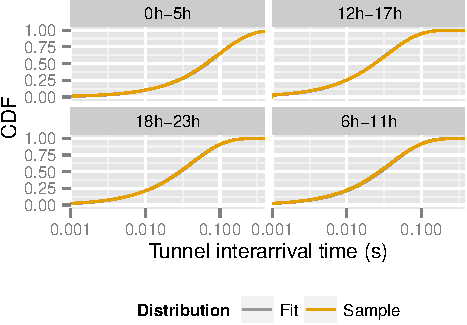
\includegraphics[width=1.0\columnwidth]{figures/R-IAT-active-fit-cdf-facets.pdf}
  \caption{Empirical and exponentially fitted CDFs of the tunnel interarrival duration by time of day. CDFs are overlapping as the coefficient of determination is close to $1$.}
  \label{fig:pdparrivalsecdf}
\end{figure}
Using this dataset, we can now compare the processes in our proposed models with the empirical distributions from actual data. First, we take a look at the tunnel interarrival time in Figure~\ref{fig:pdparrivalsecdf}.
%Tunnels can be initiated and shut down in rapid succession, thus causing the aforementioned issues in the radio network.
The arrivals show a strong diurnal effect, closely resembling patterns also present in user plane traffic.
In the data we see a decline of arrivals, i.e., longer interarrivals, late in the night and during the early morning hours with a peak rate in the afternoon and early evening.
To represent this time-of-day dependence in the model, the measurement was split into the four time slots displayed in the figure.
Each slot was then fitted with an exponential distribution with the rates $\lambda$ given in Table~\ref{tab:fits} for the four time slots.
The fitted functions match the empirical data, with some deviation present at the left tail but overall with a correlation coefficient approaching positive $1$.
\begin{figure}[htbp]
  \centering
  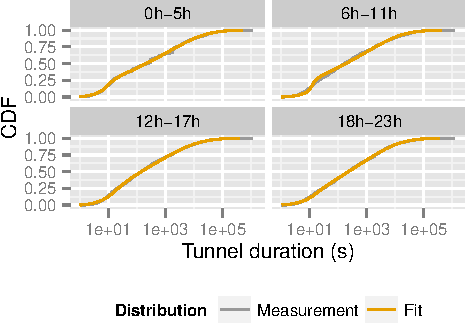
\includegraphics[width=1.0\columnwidth]{figures/timeslot-fits.pdf}
  \caption{Empirical and fitted CDFs of the tunnel duration by time of day with fitted rational functions.}
  \label{fig:fittedsdurationlots}
\end{figure}
Next, we consider the duration the \gls{PDP} Context state, which accompanies any \gls{GTP} tunnel, is held at the \gls{GGSN}.
Fig.~\ref{fig:fittedsdurationlots} shows the tunnel durations split up for the time of day. There is once again a slight diurnal effect present, albeit with shifted peaks. Longer tunnels tend to occur at night, shorter tunnels during midday.
For the model a distribution fit of the tunnel duration was also desired.
However, none of the basic probability distributions (including exponential, gamma, and Weibull distributions) fit the tunnel duration well enough.
We assume, that this can be attributed to the correlation of the tunnel duration to a large number of external factors, including user behavior, network-specific timers and procedures. All of which introduce artifacts and make it difficult to fit any distribution against.
To get some kind of approximate mathematical representation of this distribution regardless, we attempted a rational function fit using Eureqa \cite{eureqa_paper}.
%, allowing for a much closer fitting while still smoothing out some of the artifacts.
Table~\ref{tab:fits} additionally displays the generated functions which were fitted to the inverse CDF\footnote{The inverse CDF was chosen as target to be able to directly use them in the random number generator in our simulation.}. 
Both the CDFs in Fig.~\ref{fig:fittedsdurationlots} as well as the Pearson correlation coefficients confirm the goodness of the fitted functions.
\begin{table}[htbp]
  \caption{Parameters for the exponentially distributed inter-arrival times and corresponding Pearson correlation coefficients as well as the inverse functions fitted to the empirical duration distribution and correlation coefficients of the fit.}
  \label{tab:fits}
  \tabcolsep=0.11cm
  \centering
  \begin{tabu}{X[2,l]X[r]X[r]X[4.5,r]X[r]} 
  \toprule
  Time of Day & $\lambda$ & $R_{arr}$ & Inverse Fitted Duration Function & $R_{dur}$\\% \tabucline[1pt]-\everyrow{\tabucline[on 1.5pt off 2pt] -
  \midrule
  0h-5h & $10.67$ & $0.99$ & $0.91 - 60.61y - 3498.78y^3 - \frac{110.70y + 2289.94y^3}{y - 1.00}$ &  $0.99$ \\
  6h-11h & $24.53$ & $0.99$ & $1 + 117.48y - 368.64y^2 - \frac{1720.13y^4}{y - 1.00}$ & $0.99$ \\
  12h-17h & $29.25$ & $0.99$ & $0.95 + 69.49y + \frac{81146.10y^3 + 1.08\times10^6y^5}{805 - 802.01y}$ & $0.99$ \\
  18h-23h & $23.49$ & $0.98$ & $0.91 + 82.05y - \frac{2936.93y^4}{1.94y - 1.95}$ & $0.99$ \everyrow{} \\ \bottomrule
  \end{tabu}
\end{table}
